%!TEX root = ../report.tex
\chapter{Initial Experiment}
\label{ch:initial_experiment}
In the fall of 2015, we developed a state-of-the-art \ac{tsa} system based on the most common approaches within the field, outlined in Section~\ref{sec:state_of_the_art}. The system was created for the \ac{semeval} 2016 and its \ac{tsa} specific task: "Message Polarity Classification".\footnote{SemEval 2016 Task 4a, Message Polarity Classification: Given a tweet, predict whether the tweet is of positive, negative, or neutral sentiment.} The development of the system acted as both an introduction to the field of \ac{tsa} and as inspiration for the project goals listed in Section~\ref{sec:project_goals}. In this chapter the overall system architecture is described, followed by test results and results from our participation in \ac{semeval} 2016. Shorter versions of this system description previously appeared in \cite{JahFre16} and \cite{JahFre15}.

\section{Sentiment Classifier Architecture}
To solve the three-class classification problem, a general multi-class classifier, named \textit{BaseClassifier}, was created. By following a general interface, several \textit{BaseClassifier}s could be combined sequentially to create a multi-step classifier, or in parallel to create an ensemble classifier.


\section{BaseClassifier}
\label{sec:core_architecture}
The Sentiment Analysis system created was developed using the Python programming language and the Scikit-Learn machine learning framework described in Section~\ref{sec:background_scikit}. The \textit{BaseClassifier} consists of a three step process: preprocessing, feature extraction, and classification or training. The three consecutive steps are handled by the \textit{Pipeline} also described in Section~\ref{sec:background_scikit}. Each \textit{Transformer} (feature extractor) is presented with preprocessed data. The preprocessing methods used are dependent on the different \textit{Transformer}s and the features they aim to extract. The different \textit{Transformer}s and the range of preprocessors used are described later in this section. Figure~\ref{fig:core_architecture} illustrates the overall architecture of the system. \\

\begin{figure}[t]
    \begin{center}
        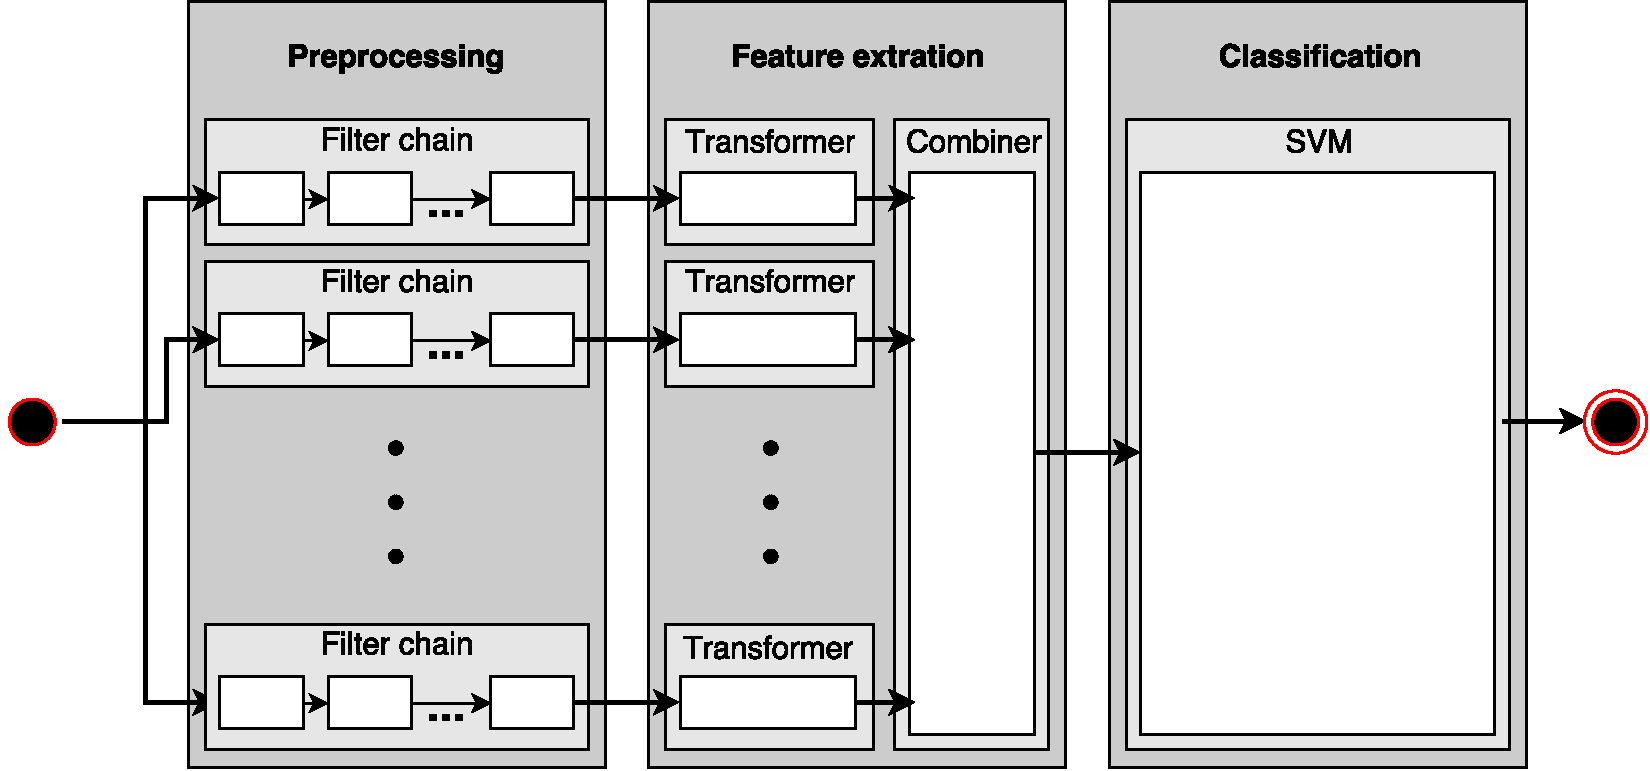
\includegraphics[width=\textwidth]{./figs/core_architecture}
    \end{center}
    \caption{Architecture of the Initial Experiment}
    \label{fig:core_architecture}
\end{figure}

The \textit{BaseClassifier} is very general. When creating a \textit{BaseClassifier} instance, it takes in a dictionary that specifies all of its parameters. The parameter dictionary includes the classifier algorithm, such as SVM, Naïve Bayes or MaxEnt, options for each of the transformers, for example $n$ value for the character and word $n$-gram transformers, or which preprocessing functions to use.

\subsection{Preprocessing}
The preprocessing step of the system modifies the raw tweets before they are passed to feature extraction, and is a necessary stage to improve the overall performance of the system. In this stage simple methods are chained together to modify raw tweets using regular expressions. Limiting each preprocessor to perform only one simple task allows for easy management of the preprocessing used by the different transformers. Table~\ref{tab:filters} lists all the basic preprocessors.

\begin{table}[t]
    \centering
    \begin{tabular}{| l | p{9.3cm} |}
        \hline
        \textbf{Filter} & \textbf{Description} \\ \hline
        %html_decode
        tokenize & Performs tweet tokenization using tokenizer by \cite{PottsTokenizer} \\ \hline
        lower\_case & Transforms all uppercase characters to lowercase \\ \hline
        no\_emotes & Replaces various emoticons with empty string \\ \hline
        no\_user & Replaces all username mentions with empty string \\ \hline
        no\_rt\_tag & Replaces all RT tags with empty string \\ \hline
        no\_url & Replaces all URLs with empty string \\ \hline
        no\_hashsign & Replaces all hash marks (\#) with empty string \\ \hline
        no\_hashtag & Replaces all hash marks along with the following tag with empty string \\ \hline
        limit\_chars & Removes all non alphabetic or space characters \\ \hline
        limit\_repeat & Limits maximum repeating of a single character to three \\ \hline
    \end{tabular}
    \caption{List of preprocessors used in the Initial Experiment}
    \label{tab:filters}
\end{table}

\subsection*{Negation Detection}
A subset of the transformers perform better when negation is identified in the tweets. Negation detection is therefore an important tweet preprocessing step performed on all tweets before being sent to negation-dependent transformers. \\

To perform negation detection, the system uses a simple approach, where $n$ words appearing after a negation cue are marked as negated by attaching ``\texttt{\_NEG}'' to the end of each word. If a punctuation mark is encountered before reaching the $n$--th word, the negation marking is stopped. By setting $n=-1$, negation marking is extended until the next punctuation or the end of the tweet. To detect the negation cues, all words in a tweet are checked against a list of negation cues. All negation cues used in our system are listed in Table~\ref{tab:negation_cues}. The negation cues were adopted from \cite{Councill10}, additionally we added common misspellings and other closely related words by looking up each negation cue in TweetNLP's word cluster, described in Section~\ref{sec:tweetnlp}.

\begin{table}[t]
    \centering
    \begin{tabular}{| l | l | l | l | l | l | l |}
        \hline
        \multicolumn{7}{|c|}{\textbf{Negation Cues}} \\ \hline
        ain't & aint & anit & can't & cannot & cant & couldn't \\ \hline
        couldnt & didn't & didnt & dnt & does'nt & doesn't & doesnt \\ \hline
        don't & dont & hadn't & hasn't & hasnt & haven't & havent \\ \hline
        havn't & havnt & isn't & isnt & lack & lacking & lacks \\ \hline
        no & nor & not & shouldn't & shouldnt & wasn't & wasnt\\ \hline
        won't & wont & wouldn't & wouldnt & \multicolumn{3}{c|}{} \\ \hline
    \end{tabular}
    \caption{List of negation cues used in the Initial Experiment}
    \label{tab:negation_cues}
\end{table}


\subsection{Feature Extraction}
\label{sec:feature_extraction}
In our system the feature extraction set is implemented as a Scikit-Learn \textit{Feature Union}, which is a collection of independent transformers (feature extractors), that builds a feature matrix for the classifier. Each feature we want to extract is represented by a \textit{Transformer}. Table~\ref{tab:feature_extractors} gives an overview of all the feature extractors used in the system.

\begin{table}[ht]
    \centering
    \begin{tabular}{| l | p{10cm} |}
        \hline
        \textbf{Features} & \textbf{Description} \\ \hline
        Word $n$-grams & Extracts TF--IDF values for combination of sequential words as described in Section~\ref{sec:background_tfidf} \\ \hline
        Char $n$-grams & Extracts TF--IDF values for combination of sequential characters \\ \hline
        Lexicon & Extracts a few values that are calculated as a function of the sentiment value of words in the tweet \\ \hline
        Word Clusters & Extracts a \textit{Bag-of-Words} model of cluster IDs for each token in the tweet \\ \hline
        Part-of-Speech & Extracts a \textit{Bag-of-Words} model of part-of-speech tags for each token in the tweet \\ \hline
        Emoticons & Extracts number of positive and negative emoticons found in the tweet \\ \hline
        Punctuation & Extracts number of repeated alphabetical and grammatical signs \\ \hline
        VADER & Extracts results from VADER sentiment analysis \\ \hline
    \end{tabular}
    \caption{List of feature extractors used in the Initial Experiment}
    \label{tab:feature_extractors}
\end{table}


\subsection*{TF--IDF Transformer}
Both \textit{Word n-grams} and \textit{Character n-grams} are realized using a \ac{tfidf} vectorizer that uses the bag of words model outlined in Section~\ref{sec:background_nlp}. Our implementation extends Scikit-Learn's default \textit{TfidfVectorizer}.


\subsection*{Lexicon Transformer}
The sentiment lexicon feature is represented by a single transformer using multiple different prior polarity sentiment lexica. The lexica used are a combination of automatic and manually annotated lexica, where some also contain sentiment scores for words in negated contexts. \\

The automatically annotated lexica used are the \textit{Sentiment140} and the \textit{HashtagSentiment} by \cite{MohammadKZ2013}, and contain sentiment scores for both unigrams and bigrams, where some are in a negated context. The unigrams and bigrams in a negated context are listed with a ``\texttt{\_NEG}'' attachment to differentiate between the two types of sentiment scores. \\

The features extracted for each tweet from these two lexica are adopted from \cite{MohammadKZ2013} and comprise:
\begin{itemize}
    \item The number of unigrams or bigrams with sentiment score $\neq0$.
    \item The sum of all sentiment scores.
    \item The highest sentiment score.
    \item The sentiment score of the last unigram or bigram.
\end{itemize}

The manually annotated lexica we used are the \textit{MPQA} by \cite{Wilson05}, the \textit{BingLiu} by \cite{Hu04}, the \textit{AFINN} by \cite{AFINN}, and the \textit{NRC Emoticon} lexicon by \cite{MohammadKZ2013}. The \textit{MPQA} and the \textit{BingLiu} lexica do not list sentiment scores for words, but instead whether a word contains positive or negative sentiment. After checking a word of a tweet against these lexica, the word is either given the score $-1$ or $+1$, for a negative or positive word sentiment, respectively. The \textit{AFINN} and the \textit{NRC Emoticon} lexica are similar to the two automatically annotated lexica described above, where each word for the \textit{AFINN} lexicon and each emoticon for the \textit{NRC Emoticon} lexicon is given a sentiment score. \\

Also for the manually annotated lexica, four features were extracted. The four features are as above, adopted from \cite{MohammadKZ2013} and comprise:
\begin{itemize}
    \item The sum of positive scores for words not in a negated context.
    \item The sum of negative scores for words not in a negated context.
    \item The sum of positive scores for words in a negated context.
    \item The sum of negative scores for words in a negated context.
\end{itemize}


\subsection*{Word Cluster Transformer}
The word cluster transformer extracts the word cluster feature by counting the occurrences of the different cluster IDs in each tweet. That is, if a word in a tweet exists in a cluster, a counter for that specific cluster ID is incremented by one. The word cluster used is described in Section~\ref{sec:tweetnlp}.

\subsection*{Part-of-Speech Transformer}
Uses the GATE TwitieTagger to assign part-of-speech tags to every token in the text, the tag occurrences are then counted and returned.

\subsection*{Punctuation Transformer}
The occurrences of continuous use of punctuation marks and characters are detected by the punctuation transformer. The feature it extracts is the number of these occurrences. 

\subsection*{Emoticon Transformer}
Similarly to the punctuation transformer, the emoticon transformer also searches for specific occurrences of characters that make up an emoticon in a tweet. For the emoticon transformer this is the use of happy and sad emoticons. The features it extracts are therefore the number of happy emoticons and the number of sad emoticons.

\subsection*{VADER Transformer}
The VADER transformer is very simple, it simply runs the VADER sentiment analysis tool, described in Section~\ref{sec:vaderSentiment}, and extracts the output from it.


\subsection{Classification}
\label{sec:arch_classification}
After all desired features have been extracted, our system uses the \ac{svm} algorithm to classify the data into one of the three classes: positive, neutral or negative. The \ac{svm} algorithm was chosen for being a state-of-the-art text classification algorithm as discussed in Section~\ref{sec:state_of_the_art}.  \\


\subsection*{Support Vector Machine}
\label{sec:svm}
The current standard incarnation of the \ac{svm} classification algorithm was proposed and formally described by \cite{VapnikCortes1995}. The algorithm takes a set of data points located in a feature space and attempts to split the feature space into optimal class segments. The attempt to split the feature space into optimal class segments is often referred to as \textit{training} the machine. When presented with a new unclassified data point, the data point is assigned the class of the class segment it is located in. \\

The spatial location of a data point is determined by the numerical value of its features. In a two dimensional scenario, a data point consists of two features; $x$ and $y$. If the data point is a representation of a sentence, $x$ could be the number of words in the sentence and $y$ the number of uppercase letters. Of course in real SA systems, the number of features will be much higher.  \\

In a simplified form, the algorithm solves a binary classification problem where the data is linearly separable. In that case the feature space is divided into two class segments. The class segments are separated by a hyperplane with the largest possible margin between the two segments --- this concept is called \textit{margin maximization}. The data points closest to the hyperplane for each class, laying on a vector parallel to it, are called \textit{support vectors}. Hence the name of the algorithm: \textit{\acl{svm}}. \\

\begin{figure}[t]
    \centering
    \begin{subfigure}[b]{0.45\textwidth}
        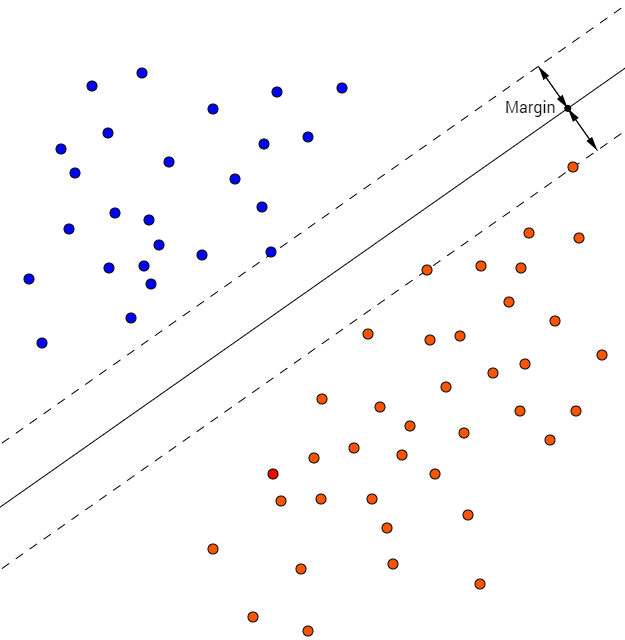
\includegraphics[width=\textwidth]{./figs/non_svm_classification_illustration}
        \caption{Non maximized margin separation}
        \label{fig:non_maximized_margin}
    \end{subfigure}
    \begin{subfigure}[b]{0.45\textwidth}
        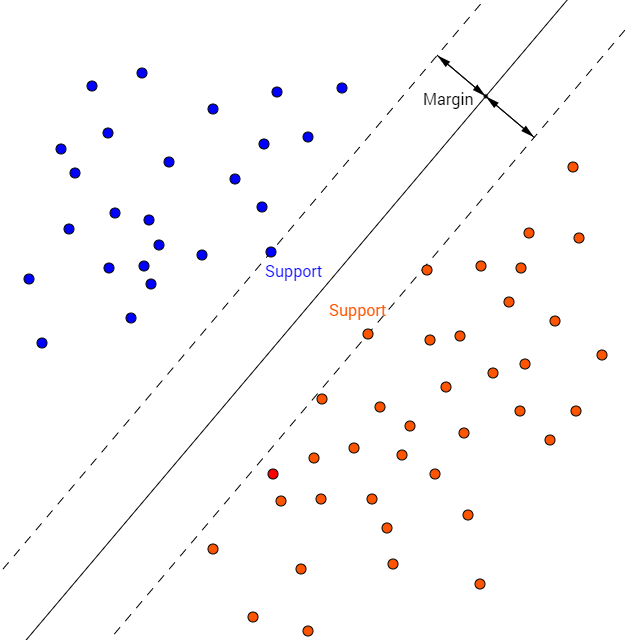
\includegraphics[width=\textwidth]{./figs/svm_classification_illustration}
        \caption{SVM maximized margin separation}
        \label{fig:svm_maximized_margin}
    \end{subfigure}
    \caption{Two possible results of linear binary classification}
    \label{fig:classification_comparison}
\end{figure}

Figure~\ref{fig:classification_comparison} illustrates two different ways of splitting the data into two classes. Figure~\ref{fig:non_maximized_margin} shows a non-maximized margin split, while Figure~\ref{fig:svm_maximized_margin} follows the \ac{svm} algorithm of finding the support vectors that result in the largest margin between the two segments. \\

The algorithm can also be used if linear separation of the training data is impossible. This could either be achieved by allowing misclassified points and introducing a slack variable, or by using the \textit{kernel trick}. In the first approach the misclassified points are assigned a penalty related to the distance away from the support vector of their class segment. The longer the distance, the higher the penalty. The penalty comes in the form of a positive slack variable, which governs the trade-off between misclassified points and the margin. \\

By using the \textit{kernel trick}, the data is mapped onto a higher dimensional space where it becomes linearly separable. This is done by applying a \textit{kernel function} to the data. The most popular kernel functions are the Radial Basis, the Polynomial and Sigmoidal kernels. The in-depth explanation of \ac{svm} by \cite{Fletcher09} states that finding the right kernel function is more of an art than an exact science. It often comes down to trial and error. \\

\begin{figure}[t]
    \centering
    \begin{subfigure}[b]{0.45\textwidth}
        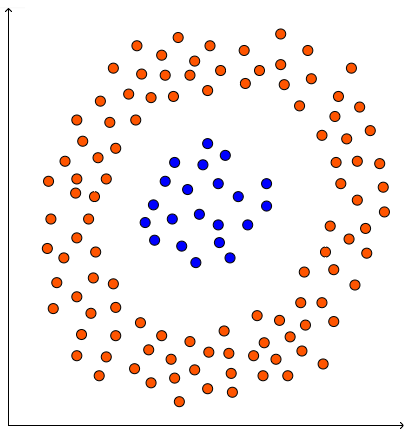
\includegraphics[width=\textwidth]{./figs/non_linearly_separable_classes}
        \caption{Before application of \textit{kernel trick}}
        \label{fig:non_linearly_separable_2d}
    \end{subfigure}
    \begin{subfigure}[b]{0.45\textwidth}
        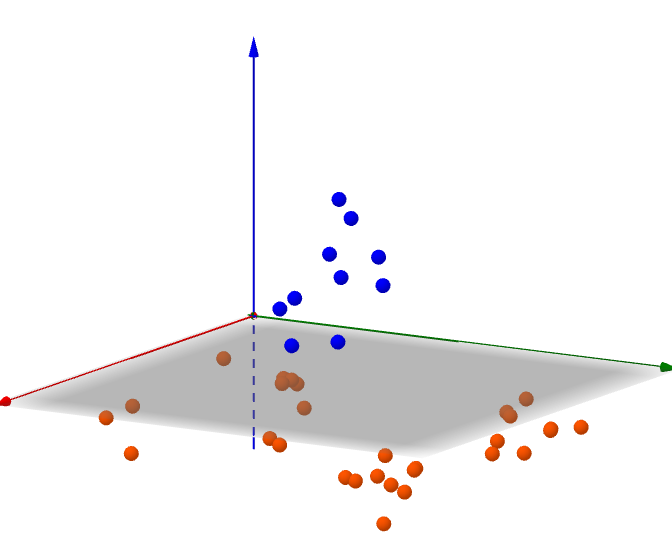
\includegraphics[width=\textwidth]{./figs/non_linearly_separable_classes_higher_dimension}
        \caption{After application of \textit{kernel trick}}
        \label{fig:non_linearly_separable_3d}
    \end{subfigure}
    \caption{\textit{Kernel trick} applied to a non-linearly separable dataset}
    \label{fig:non_linearly_separable_classes}
\end{figure}

Figure~\ref{fig:non_linearly_separable_2d} shows a dataset with a clear pattern which is not linearly separable. Figure~\ref{fig:non_linearly_separable_3d} shows the same dataset after being transformed by a kernel function to 3-dimensional space. The items occupy the same positions on the $xy$-plane, but are separable along the $z$-axis. \\

The \ac{svm} algorithm can also be applied to classification problems with more than two classes. To solve the multi-class classification problem, two methods, One-vs-All and One-vs-One, are commonly used. Both methods use a set of binary \ac{svm} classifiers and are thoroughly explained by \cite{HsuLin02}. Popular implementations of the \ac{svm} algorithm includes solving quadratic programming problems using a sequential minimal optimization algorithm invented by \cite{Platt98}.


\subsection*{Realization of the Classifier}
The classifier was realized using the Scikit-Learn framework which includes a series of \ac{svm} implementations. We chose the SVC variant, also known as C-Support \ac{svm} classifier, which is based around the idea of setting a constant $C$ that will be used to penalize incorrectly classified instances. High $C$ values will create a narrower margin, which will be able to classify more training elements correctly, but may also lead to overfitting. Therefore, it is desirable to perform some kind of parameter optimization to find the optimal $C$ value. For multi-class classification, Scikit-Learn uses the One-vs-One method, with a run time complexity quadratic to number of elements. However, this will not be a problem for the relatively small (under 10\thinspace000 elements) SemEval datasets. 


\section{Combining BaseClassifiers}
\subsection{Multi-Step Classifier}
\label{sec:multi_step_classifier}

\begin{figure}[t]
    \begin{center}
        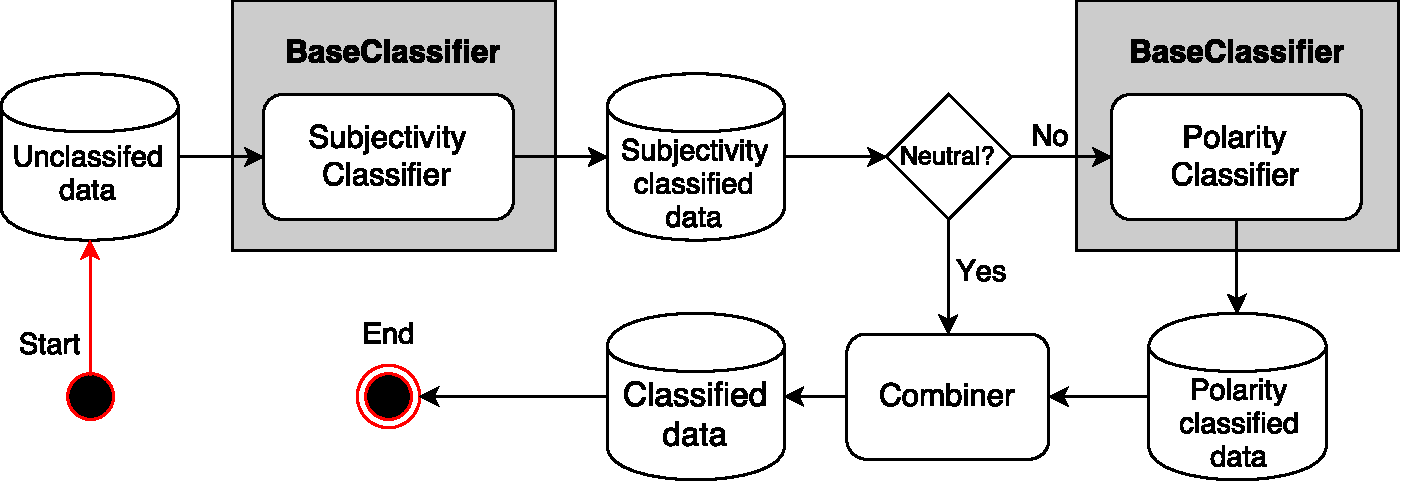
\includegraphics[width=\textwidth]{./figs/data_flow}
    \end{center}
    \caption{Data flow in the two-step classifier}
    \label{fig:data_flow}
\end{figure}

A single \textit{BaseClassifier} acts as a one-step classifier, but by chaining \textit{BaseClassifier}s sequentially, we can create a multi-step classifier. Each classifier can be trained independently on different data thereby learning a different classification function. Figure~\ref{fig:data_flow} illustrates how chaining of two \textit{BaseClassifier}s can create a two-step classifier. The first \textit{BaseClassifier} is trained only on data labeled as subjective or objective, while the second \textit{BaseClassifier} trains only on subjective data, labeled positive or negative. When classifying, if the first \textit{BaseClassifier} classifies an instance as subjective, the instance is forwarded to the second \textit{BaseClassifier} to determine if the instance is positive or negative. The results from both classifiers are then combined together and the final classifications are returned.

\subsection{Ensemble Classifier}
By combining the \textit{BaseClassifier}s in parallel, we can create an ensemble of classifiers. Each of the classifiers is independent of the others and all classify the same instances. At the end, the classifiers take a vote to decide on the final classification of the instance. Because the \textit{BaseClassifier}s are so general, it is possible to create \textit{BaseClassifier}s that extract different features, do different preprocessing and use different classification algorithms; we could combine them to create an ensemble system. 


\section{Results}
\label{sec:init_experiment_results}

\subsection{Test Results}
\label{sec:test_results}
In order to thoroughly test our system and its components, two main tests were conducted. A performance test of our final system with optimal parameters on all datasets, comparing the performance of our system against previous \ac{ntnu} developed \ac{tsa} systems, and an ablation study to identify the importance of the different features used in our system. 

\subsection*{Classifier Performance}
 Our \ac{tsa} system was trained on the \textit{\ac{semeval} 2013-train} training set, using the optimal parameters identified through a grid search, and tested on the \textit{\ac{semeval} 2013-test} and the \textit{\ac{semeval} 2014-test} test sets before being scored using the scoring metrics described in Section~\ref{sec:classification_scoring_metrics}. The results are shown in Table~\ref{tab:system_comparison} together with the results of the systems we aimed to improve. \\
 
 The performance of our system, compared to the previously \ac{ntnu} developed \ac{tsa} systems of \citep{FaretReitan, ReitanEtAl15} and \citep{SelmerBrevik, SelmerEtAl13} is very good. On the \textit{2013-test} set, we can see that our system performs better than \citeauthor{FaretReitan} and a lot better than \citeauthor{SelmerBrevik}. On the \textit{2014-test} set our system performs identical to \citeauthor{FaretReitan}, while still performing better than \citeauthor{SelmerBrevik}. However, an important aspect to notice is the execution time. Although we were not able to replicate the results of \citeauthor{FaretReitan} by running their system, we got a rough estimate of their execution time. On the \textit{2013-test} set their execution time was 180 seconds against our 74, and on the \textit{2014-test} set their time was 93 against our 41. Even though these execution time estimates are unofficial, they still indicate a reduction in execution time from their system to ours. Compared to the execution time of \cite{SelmerBrevik} our system is still quite slow, but the simplicity of their system also leads to a significantly lower performance.
 

\begin{table}[t]
    \centering
    \begin{tabular}{l|c|c|c|c|c|}
        \cline{2-6}
        & \textbf{System} & \textbf{Precision} & \textbf{Recall} & \textbf{F1-Score} & \textbf{Time} \\
        \cline{1-6}
        \multirow{3}{*}{\rot{2013}} & \citeauthor{SelmerBrevik} & 0.6787 & 0.6644 & 0.6482 & 0.36 \\
        \cline{2-6}
        & \citeauthor{FaretReitan} & 0.731 & 0.697 & 0.688 & \textasciitilde{}180 \\
        \cline{2-6}
        & \textbf{Initial Experiment} & 0.7209 & 0.7120 & 0.7073 & 74.01 \\
        \hhline{======|}
        
        \multirow{3}{*}{\rot{2014}} & \citeauthor{SelmerBrevik} & 0.7071 & 0.6667 & 0.6614 & 0.17 \\
        \cline{2-6}
        & \citeauthor{FaretReitan} & 0.738 & 0.684 & 0.684 & \textasciitilde{}93 \\
        \cline{2-6}
        & \textbf{Initial Experiment} & 0.7091 & 0.6832 & 0.6847 & 41.38 \\ \hline
    \end{tabular}
    \caption{Initial Experiment performance comparison}
    \label{tab:system_comparison}   
\end{table}

\subsection*{Ablation Study}
\label{sec:ablation_study}
In order to detect the overall importance or impact each feature has on our \ac{tsa} system, we conducted a simple ablation study. This was done by removing each feature in turn and checking how the performance of the system was affected. The results of the ablation study are shown in Table~\ref{tab:ablation_study}. \\

\begin{table}[t]
    \centering
    \begin{tabular}{|l|c|c|}
        \hline
        \textbf{Features} & \textbf{2013-test} & \textbf{2014-test} \\ \hline
        All                             & 0.7073 & 0.6847 \\ \hline
        All - Word $n$-grams            & 0.7050 & 0.6833 \\
        All - Character $n$-grams       & 0.6992 & 0.6812 \\
        All - Both $n$-grams            & 0.6948 & 0.6784 \\ \hline
        All - Automatic Lexica          & 0.7031 & 0.6888 \\
        All - Manual Lexica             & 0.7005 & 0.6905 \\
        All - All Sentiment Lexica      & 0.6862 & 0.6818 \\ \hline
        All - Word Clusters             & 0.7072 & 0.6825 \\ \hline
        All - Part-of-Speech tag counts & 0.7080 & 0.6879 \\
        All - Punctuation counts        & 0.7128 & 0.6946 \\
        All - Emoticons counts          & 0.7028 & 0.6826 \\ 
        All - All counts                & 0.7069 & 0.6787 \\ \hline
        All - VADER Sentiment           & 0.6960 & 0.6796 \\ \hline
    \end{tabular}
\caption[Ablation study results for the Initial Experiment]{Ablation study results. All - F means all features except for F. All values are $F_1$-scores.}
    \label{tab:ablation_study}   
\end{table}

As we can see, the single most important feature is the Sentiment Lexica. On the \textit{2013-test} set the accuracy of the system is reduced from 0.7073 to 0.6862 when the feature is removed. The effect of removing the Sentiment Lexica feature when tested on the \textit{2014-test} set is not as apparent. A possible cause of the difference in performance impact may be that most of the Sentiment Lexica used were created at the same time as the \textit{2013-test} set, and could possibly better reflect the language in that period of time. For the \textit{2014-test} it is less clear which feature is the best, collectively $n$-grams and all counts perform better, but VADER Sentiment is the single most important feature, reducing the accuracy from 0.6847 to 0.6796 when being removed. On the \textit{2013-test} set on the other hand, the VADER Sentiment feature does not have the same impact, but is still the second most important single feature. As VADER Sentiment was created in 2014, the cause of this difference may also be a change in how the language is used and that VADER Sentiment better reflects the language in 2014.  \\

The second most important features are the $n$-gram features. The removal of both character $n$-grams and word $n$-grams leads to a significant degradation in performance on both datasets. \\

Another interesting result is the impact of the features: Part-of-Speech counts and Punctuation counts. On both the \textit{2013-test} and the \textit{2014-test} sets, removal of those features causes slight improvement in performance, but when removed together with the Emoticon counts, the degradation in performance is larger than the performance degradation caused by only removing the Emoticon counts feature. A possible cause for this is that the classifier finds a pattern between all three of the counts that disappears when one of them is removed.


\subsection{SemEval 2016 Results}
We participated with the Initial Experiment system in \ac{semeval} 2016 subtask 4a: "Message Polarity Classification" under the team name \textit{NTNUSentEval} and ended up on the 11th place out of 34 competing systems, as shown in Table~\ref{tab:semeval_results}. \\

Our system was ranked as number 1 on the SMS dataset and as number 3 on the Live-Journal dataset. On the remaining datasets containing tweets, the system was ranked between 10th-13th place. The reason why our system performed so well on SMS and Live-Journal messages is unclear. A possible explanation may be that our system was only trained on the \textit{2013-train} dataset, while more than half the teams participating in SemEval 2016 also used large external tweet datasets, which could improve their performance on Twitter data, but also lead to worse performance on out-of-domain data. 

\glsresetall